\chapter{HASIL DAN PEMBAHASAN}
\label{chap:resultsandiscussion}

% Ubah bagian-bagian berikut dengan isi dari pengujian dan analisis

Bagian ini membahas dan menunjukkan hasil dari pengujian dan analisis kami pada pelatihan model robot humanoid, perbandingan model manusia, dan juga membandingkan kecocokan antara mereka.
Semua pengujian dilakukan menggunakan robot Ichiro di Laboratorium \emph{Robot Cerdas} dengan spesifikasi komputer seperti yang terlihat pada Tabel \ref{tb:computerspecichiro}.

\def\arraystretch{1.5}
\begin{longtable}{|c|c|}
  \caption{Spesifikasi Komputer pada robot Ichiro.}
  \label{tb:computerspecichiro}\\
  \hline
  OS      & Ubuntu 20.04.2 LTS \\
  \hline
  CPU     & Intel i5-10210U (8) @ 4.200GHz \\
  \hline
  GPU     & Intel UHD Graphics  \\
  \hline
  RAM     & 3636 MiB \\
  \hline
\end{longtable}


\section{Statistik Dataset Baru}
\label{sec:new-dataset-statistics}

Dataset baru ini merupakan kombinasi dari dataset HumanoidRobotPose dan dataset milik kami sendiri. Gambar \ref{fig:nimbro-statistics} menunjukkan statistik untuk dataset HumanoidRobotPose, sedangkan Gambar \ref{fig:new-dataset-statistics} menunjukkan statistik untuk dataset baru tersebut.
\begin{figure}[ht]
  \centering
  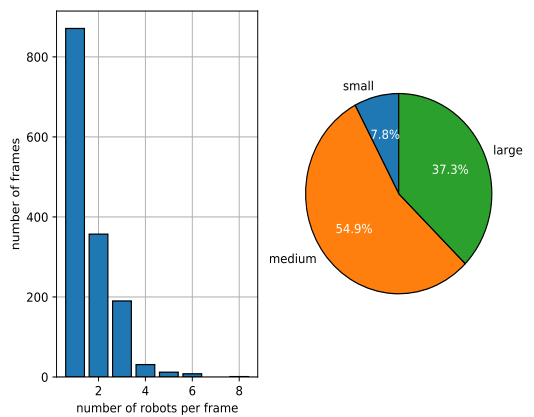
\includegraphics[scale=0.8]{gambar/old_dataset.png}
  \caption{Statistik HumanoidRobotPose.}
  \label{fig:nimbro-statistics}
\end{figure}
Keanekaragaman jumlah robot tiap gambar diilustrasikan di sebelah kiri, sedangkan proporsi skala robot ditunjukkan di sebelah kanan. Definisi skala kecil, sedang, dan besar sesuai dengan dataset COCO.
Sebagian besar data yang ditambahkan adalah satu robot (dari sekitar 850 menjadi 1700) tiap gambar dan hanya beberapa yang memiliki dua robot (dari sekitar 380 menjadi 430) dengan skala besar, yaitu (luas area \textgreater 96\textsuperscript{2}).
Ini didasarkan pada persyaratan sistem yang hanya membutuhkan estimasi pose untuk satu robot dan karena jarak antara kamera dan robot tidak terlalu jauh, objek robot dalam gambar sebagian besar adalah skala besar.
\begin{figure}[ht]
  \centering
  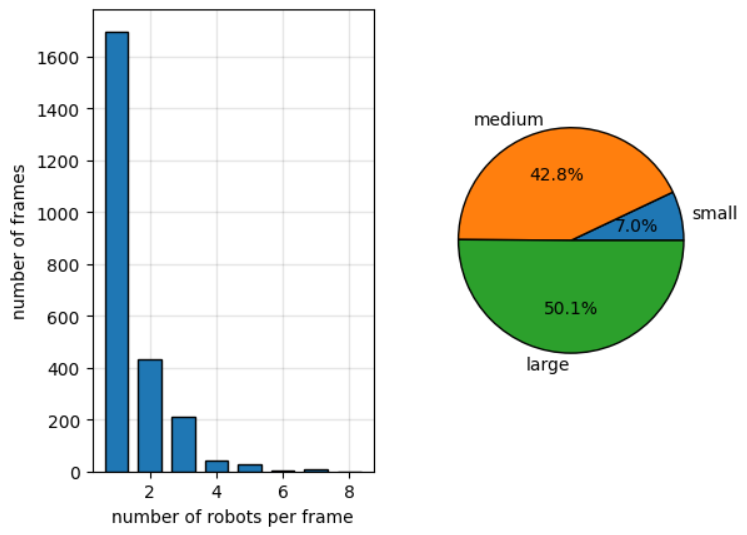
\includegraphics[scale=0.63]{gambar/new_dataset.png}
  \caption{Statistik Dataset Baru.}
  \label{fig:new-dataset-statistics}
\end{figure}


\section{Hasil Pelatihan Model Robot}
\label{sec:robotmodeltrainingresult}

Bagian ini menampilkan grafik pelatihan, metrik evaluasi tentang tiga model, dan pengujian yang kami lakukan seperti visualisasi hasil deteksi dan waktu inferensi.
Gambar \ref{fig:nimbro-training-graphics}, \ref{fig:rcnn-training-graphics}, dan \ref{fig:yolo-training-graphics} menunjukkan grafik untuk \textit{loss} pelatihan (di sebelah kiri) dan \textit{loss} validasi (di sebelah kanan).
Grafik \textit{loss} pelatihan menunjukkan tren nilai \textit{loss} terhadap epoch atau iterasi saat pelatihan. Ini mencerminkan seberapa baik model belajar pada data pelatihan.
Di sisi lain, grafik loss validasi menunjukkan tren nilai \textit{loss} terhadap epoch atau iterasi saat validasi. Ini memberikan perkiraan seberapa baik model menggeneralisasi data yang belum pernah dilihat sebelumnya.
\begin{figure}[ht]
  \centering
  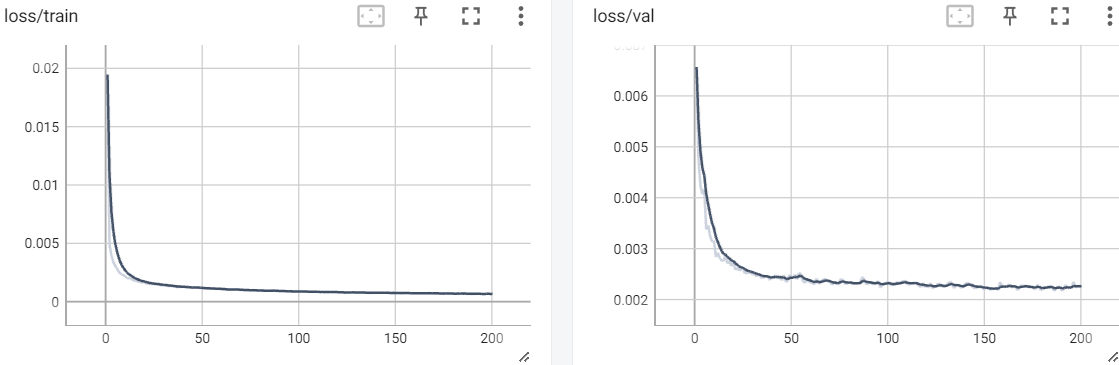
\includegraphics[scale=0.65]{gambar/loss-nimbro.png}
  \caption{Grafik Pelatihan Nimbro.}
  \label{fig:nimbro-training-graphics}
\end{figure}
\textit{Loss} pelatihan dan \textit{loss} validasi pada model NimbRo mengalami penurunan dari 0,02 menjadi 0,0006 dan dari 0,0065 menjadi 0,002. Dari Gambar \ref{fig:rcnn-training-graphics}, kita juga dapat mengetahui bahwa \textit{loss} pelatihan dan \textit{loss} validasi pada Keypoint RCNN mengalami penurunan dari 6,991 menjadi 2,634 dan dari 5,926 menjadi 3,439.
Awalnya, \textit{loss} pelatihan tinggi karena parameter model diinisialisasi secara acak dan model belum belajar untuk membuat prediksi yang akurat. Seiring berjalannya waktu, \textit{loss} akan mengalami penurunan, menunjukkan bahwa model sedang belajar dan meningkatkan performanya.
\textit{Loss} pelatihan secara bertahap menurun dan pada akhirnya stabil, ini menunjukkan bahwa model telah konvergen dan pelatihan tidak perlu dilanjutkan.
Seperti \textit{loss} pelatihan, awalnya \textit{loss} validasi relatif tinggi. Seiring model belajar dari data pelatihan, \textit{loss} validasi seharusnya mengalami penurunan, menunjukkan peningkatan kemampuan generalisasi model. \textit{Loss} validasi secara bertahap menurun dan stabil pada akhirnya.
Namun, Gambar \ref{fig:yolo-training-graphics} menunjukkan bahwa terjadi \textit{overfitting} saat melatih YOLO-pose. Hal ini ditunjukkan oleh grafik salah satu \textit{loss} validasi (\textit{loss} bounding box) yang meningkat, bukannya secara bertahap menurun. Hal ini terjadi karena biasanya YOLO membutuhkan jumlah data yang besar, namun dalam studi ini, kami hanya memiliki dataset kecil untuk pelatihan.
Sebagai contoh, saat melatih deteksi \textit{keypoint} manusia dengan dataset COCO 2017, data pelatihan terdiri dari 57 ribu gambar, sedangkan validasi dan tes terdiri dari 5 ribu dan 20 ribu gambar secara berturut-turut \parencite{maji2022yolopose}.
Kami tidak menampilkan total \textit{loss} validasi karena perhitungannya masih salah (belum menjumlahkan semua \textit{loss}) sehingga visualisasi grafiknya juga tidak benar.
\begin{figure}[ht]
  \centering
  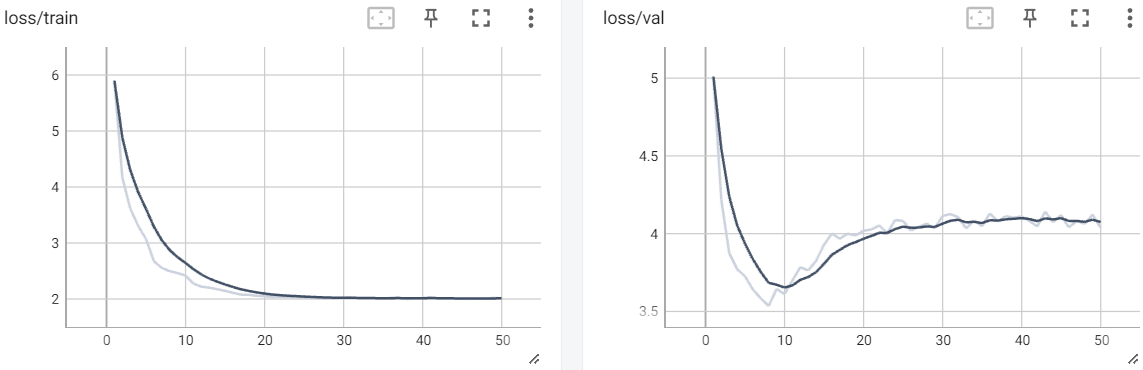
\includegraphics[scale=0.65]{gambar/loss-rcnn.png}
  \caption{Grafik Pelatihan Keypoint RCNN.}
  \label{fig:rcnn-training-graphics}
\end{figure}
\begin{figure}[ht]
  \centering
  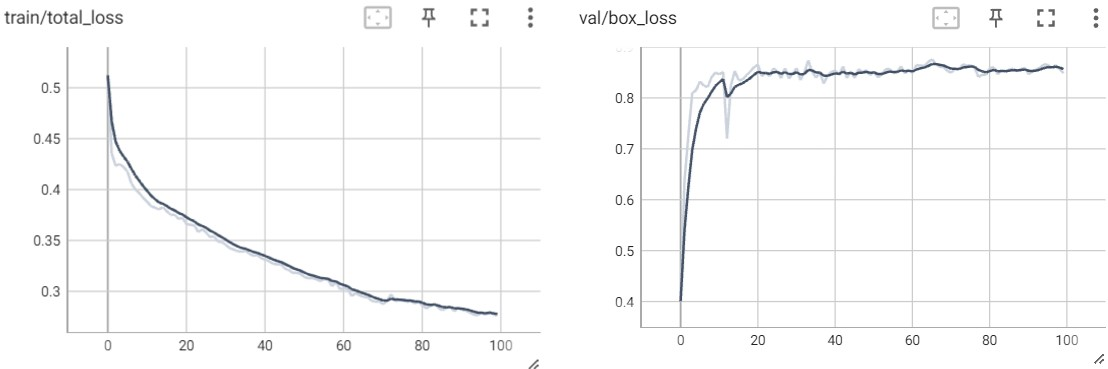
\includegraphics[scale=0.5]{gambar/loss-yolo.jpg}
  \caption{Grafik Pelatihan YOLO-pose.}
  \label{fig:yolo-training-graphics}
\end{figure}

Untuk metrik evaluasi, Model NimbRo dan Keypoint RCNN menggunakan \textit{Object Keypoint Similarity} (OKS) dengan konstanta per-keypoint sama dengan 0,4 untuk semua keypoints.
YOLO juga menggunakan OKS yang mengikuti metrik evaluasi standar estimasi pose COCO.
Dalam tugas deteksi \textit{keypoint}, presisi dan \textit{recall} umumnya digunakan sebagai metrik utama karena metrik ini mengukur kualitas prediksi (presisi mengukur proporsi keypoints yang diprediksi dengan benar dari semua prediksi keypoints dan recall mengukur proporsi keypoints yang diprediksi dengan benar dari semua \textit{ground truth} sebenarnya).
Sementara itu, akurasi bukan metrik yang relevan dalam deteksi keypoints karena tidak secara efektif mencerminkan sifat tugas tersebut.
Tugas tersebut berfokus pada lokalisisasi dan identifikasi keypoints dalam sebuah gambar, bukan mengklasifikasikan seluruh gambar atau memprediksi kategori diskrit. Oleh karena itu, mengukur akurasi yang umumnya mengevaluasi keseluruhan kebenaran dalam tugas klasifikasi mungkin tidak memberikan wawasan yang bermakna untuk tugas ini.
Selain itu, jika kita ingin mendapatkan akurasi, kita perlu mengetahui nilai \textit{True Negative} (TN). Dikarena deteksi keypoints bukan tugas klasifikasi biner (seperti mengklasifikasikan keberadaan atau ketiadaan keypoints), menentukan \textit{True Negative} juga merupakan tantangan tersendiri. Oleh karena itu, konsep \textit{True Negative} tidak secara langsung dapat diterapkan atau relevan dalam konteks ini.

Hasil pada test set dilaporkan dalam Tabel \ref{tb:result-on-test-set}. Dapat dilihat bahwa Keypoint RCNN unggul dalam semua metrik kecuali untuk skala sedang.
Selain itu, Keypoint RCNN menunjukkan hasil deteksi terbaik seperti yang ditunjukkan dalam Tabel \ref{tb:robotmodelcomparisondetectionresults}, diikuti oleh Model NimbRo dan YOLO-pose.
Terakhir, Model NimbRo kemungkinan paling cocok untuk diterapkan pada sistem \textit{real-time} karena memiliki waktu inferensi terendah seperti yang ditunjukkan dalam Tabel \ref{tb:inferencerobot}.
Namun, karena dalam mode \textit{PLAY}, kita dapat melakukan estimasi pose baik untuk manusia maupun robot humanoid pada akhir dan bukan secara langsung.
Kami memutuskan untuk menyimpan gambar terlebih dahulu dan melakukan perbandingan pose kemudian. Karena kami lebih mementingkan model dengan performa lebih baik dibangding model dengan waktu inferensi lebih cepat, maka model Keypoint RCNN cocok untuk penelitian ini.

\begin{longtable}{|L{1.5cm}|c|c|c|c|c|c|c|c|c|c|}
  \caption{Hasil pada Test Set.}
  \label{tb:result-on-test-set}\\
  \hline
  \rowcolor[HTML]{C0C0C0}
  \textbf{Model} & \textbf{AP} & \textbf{AP\textsubscript{50}} & \textbf{AP\textsubscript{75}} & \textbf{AP\textsubscript{M}} & \textbf{AP\textsubscript{L}} & \textbf{AR} & \textbf{AR\textsubscript{50}} & \textbf{AR\textsubscript{75}} & \textbf{AR\textsubscript{M}} & \textbf{AR\textsubscript{L}} \\
  \hline
  NimbRo Model & 0.828       & 0.879                         & 0.840                         & \textbf{0.886}                       & 0.864                        & 0.836       & 0.884                         & 0.849                         & 0.895                        & 0.872 \\
  \hline                        
  Keypoint RCNN  & \textbf{0.879}       & \textbf{0.936}                         & \textbf{0.904}                         & 0.859                        & \textbf{0.937}                       & \textbf{0.925}       & \textbf{0.973}                         & \textbf{0.944}                         & \textbf{0.936}                        & \textbf{0.955} \\
  \hline                        
  YOLO-pose      & 0.849       & 0.838                         & -                             & -                            & -                            & 0.814       & -                             & -                             & -                            & - \\
  \hline
\end{longtable}

\def\arraystretch{1.5}
\begin{longtable}{|c|c|c|}
  \caption{Waktu Inferensi Model Robot \textit{Humanoid}.}
  \label{tb:inferencerobot}\\
  \hline
  \rowcolor[HTML]{C0C0C0}
  \textbf{Model}    & \textbf{PyTorch (s)} & \textbf{OpenVINO (s)}\\
  \hline
  NimbRo's Model & 0.4 - 0.5 & 0.15 - 0.2 \\
  \hline
  Keypoint RCNN  & 3.5 - 4.0 & 1.25 \\
  \hline
  YOLO-pose      & 0.7 - 0.75& 0.27 - 0.3 \\
  \hline
\end{longtable}

\newpage
\def\arraystretch{0.5}
\begin{longtable}{|c|c|c|}
  \caption{Perbandingan Hasil Deteksi Model untuk Robot.}
  \label{tb:robotmodelcomparisondetectionresults}\\
  \hline
  \rowcolor[HTML]{C0C0C0}
  \textbf{NimbRo's Model}    & \textbf{Keypoint RCNN} & \textbf{YOLO-pose}\\
  \hline
  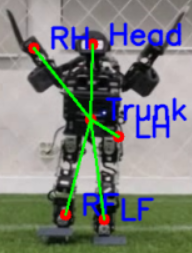
\includegraphics[scale=0.85]{gambar/nimbro-1.png} & 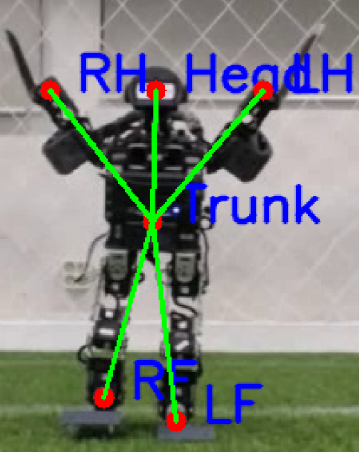
\includegraphics[scale=0.48]{gambar/rcnn-1.png} & 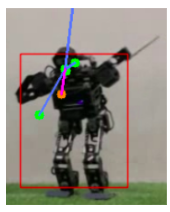
\includegraphics[scale=0.66]{gambar/yolo-1.png} \\
  \hline
  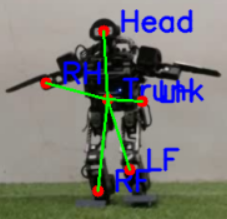
\includegraphics[scale=0.85]{gambar/nimbro-2.png} & 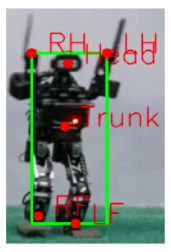
\includegraphics[scale=0.49]{gambar/rcnn-2.png} & 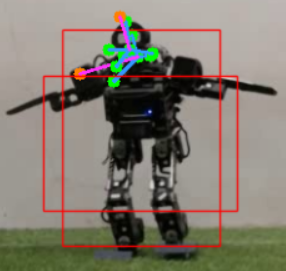
\includegraphics[scale=0.68]{gambar/yolo-2.png} \\
  \hline
  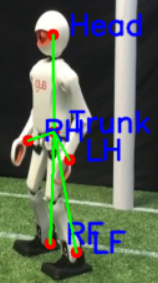
\includegraphics[scale=0.85]{gambar/nimbro-3.png} & 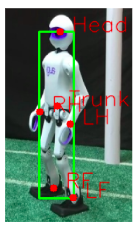
\includegraphics[scale=0.49]{gambar/rcnn-3.png} & 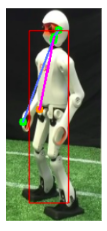
\includegraphics[scale=0.67]{gambar/yolo-3.png} \\
  \hline
\end{longtable}


\section{Perbandingan Model Manusia}
\label{sec:humanmodelcomparison}
  
Berdasarkan penelitian yang dilakukan oleh \parencite{bazarevsky2020}, mereka membandingkan tiga model yang berbeda: BlazePose Lite, BlazePose Full, dan OpenPose (hanya bagian tubuh). Mereka menguji model-model tersebut pada AR Dataset dan Yoga Dataset.
Sebagai metrik evaluasi, mereka menggunakan \textit{Percent of Correct Points} dengan toleransi 20\% (PCK@0.2) (di mana titik dianggap terdeteksi dengan benar jika kesalahan Euclidean 2D-nya lebih kecil dari 20\% dari ukuran torso orang yang bersangkutan).
BlazePose menunjukkan performa yang sedikit lebih buruk dibandingkan model OpenPose pada dataset AR, tetapi BlazePose Full unggul dibandingkan OpenPose pada kasus penggunaan Yoga/Fitness.
Perlu diperhatikan bahwa dalam penelitian ini, kami menggunakan BlazePose Full karena secara \textit{default} nilai argumen \emph{model complexity} adalah 1 dalam MediaPipe API. Mediapipe menyediakan tiga model BlazePose: BlazePose Lite, BlazePose Full, dan BlazePose Heavy. Akurasi landmark pose serta latensi inferensinya meningkat seiring dengan kompleksitas model.
Tabel \ref{tb:yoloandmediapipecomparison} menunjukkan perbandingan antara YOLO-pose dan MediaPipe Pose, dan berdasarkan kebutuhan kami untuk hanya mendeteksi satu orang, MediaPipe seharusnya menjadi pilihan terbaik untuk penelitian ini.

\def\arraystretch{1.5}
\begin{longtable}{|L{3cm}|L{5cm}|L{5cm}|}
  \caption{Perbandingan YOLO-pose dan MediaPipe Pose.}
  \label{tb:yoloandmediapipecomparison}\\
  \hline
  \rowcolor[HTML]{C0C0C0}
  \textbf{Features}    & \textbf{YOLO-pose} & \textbf{MediaPipe Pose}\\
  \hline
  Topology             & 17 Keypoints COCO  & 33 Keypoints COCO \\
  \hline
  Workflow             & Detection runs for all frames & Detection runs once followed by tracker until occlusion occurs \\
  \hline
  GPU support          & Support for both CPU and GPU & Only CPU \\
  \hline
  Number of persons    & Multi-person & Single person \\
  \hline
\end{longtable}

\begin{longtable}{|c|c|c|}
  \caption{Waktu Inferensi Model Manusia.}
  \label{tb:inferencehuman}\\
  \hline
  \rowcolor[HTML]{C0C0C0}
  \textbf{Model}    & \textbf{Inference Time (s)} \\
  \hline
  Mediapipe   & 0.15 - 0.2\\
  \hline
  OpenPose    & 1 - 2\\
  \hline
  YOLO-Pose   & 0.7 - 0.75\\
  \hline
\end{longtable}

\section{Membandingkan Kecocokan Pose Antara Manusia dan Robot \textit{Humanoid}}
\label{sec:comparingsuitabilityresults}

Dengan menggunakan metode yang dijelaskan di Bagian \ref{sec:comparing-keypoints}, kami mendapatkan hasil dari perbandingan pose manusia dan pose robot dalam persentase.
Dua gambar tersebut dapat dilihat di bawah ini, pada Gambar \ref{fig:comparingb}, manusia melakukan gerakan yang lebih mirip dengan robot daripada pada Gambar \ref{fig:comparinga}.
Oleh karena itu, hasil perbandingan dari Gambar \ref{fig:comparingb} lebih tinggi yaitu 91\% dibandingkan Gambar \ref{fig:comparinga} yang hanya 79\%.
Hal ini menunjukkan bahwa sistem dapat memberikan penilaian yang akurat antara pose manusia dan pose robot.
Selanjutnya, Gambar \ref{fig:comparisongtandresult} menunjukkan perbandingan antara \textit{ground truth} dan hasil deteksi menggunakan Keypoint RCNN untuk setiap jenis robot dalam dataset yang baru
(sisi kiri adalah ground truth dan sisi kanan adalah hasil deteksi).

\begin{figure}
  \centering
  \begin{subfigure}[b]{0.45\textwidth}
      \centering
      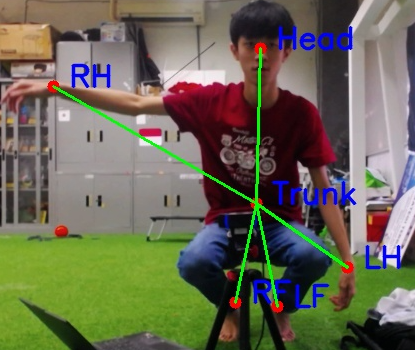
\includegraphics[width=\textwidth]{gambar/human_10_result.jpg}
      \caption{Citra Manusia}
      \label{fig:humanimagea}
  \end{subfigure}
  \hfill
  \begin{subfigure}[b]{0.45\textwidth}
      \centering
      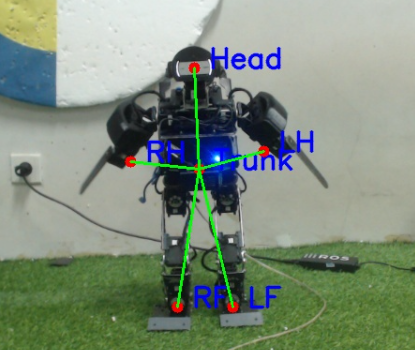
\includegraphics[width=\textwidth]{gambar/robot_6_result.jpg}
      \caption{Citra Robot}
      \label{fig:robotimagea}
  \end{subfigure}
     \caption{Membandingkan Pose Robot \textit{Humanoid} dan Pose Manusia.}
     \label{fig:comparinga}
\end{figure}

\begin{figure}
  \centering
  \begin{subfigure}[b]{0.45\textwidth}
      \centering
      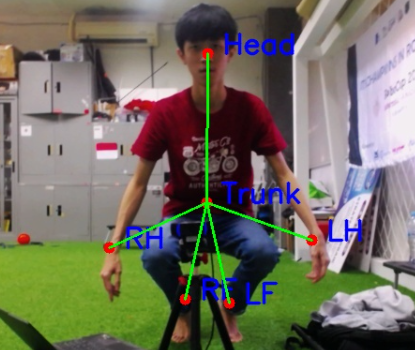
\includegraphics[width=\textwidth]{gambar/human_6_result.jpg}
      \caption{Citra Manusia}
      \label{fig:humanimageb}
  \end{subfigure}
  \hfill
  \begin{subfigure}[b]{0.45\textwidth}
      \centering
      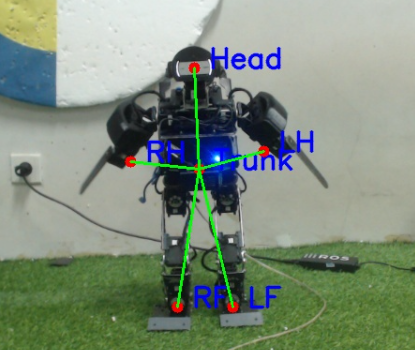
\includegraphics[width=\textwidth]{gambar/robot_6_result.jpg}
      \caption{Citra Robot}
      \label{fig:robotimageb}
  \end{subfigure}
     \caption{Membandingkan Pose Robot \textit{Humanoid} dan Pose Manusia.}
     \label{fig:comparingb}
\end{figure}

\begin{figure}
  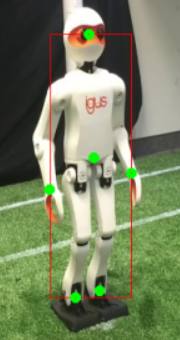
\includegraphics[width=.15\textwidth]{gambar/comp_with_gt/robot_1_gt.png}
  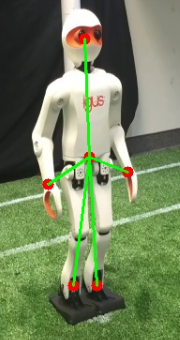
\includegraphics[width=.15\textwidth]{gambar/comp_with_gt/robot_1_res.png} \hfill%
  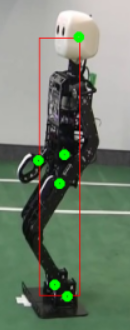
\includegraphics[width=.113\textwidth]{gambar/comp_with_gt/robot_2_gt.png}
  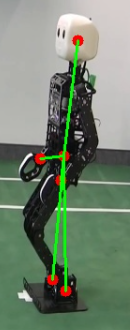
\includegraphics[width=.113\textwidth]{gambar/comp_with_gt/robot_2_res.png} \hfill%
  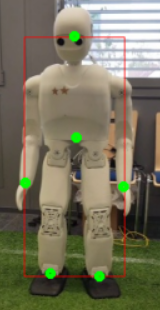
\includegraphics[width=.15\textwidth]{gambar/comp_with_gt/robot_3_gt.png}
  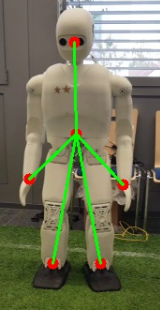
\includegraphics[width=.15\textwidth]{gambar/comp_with_gt/robot_3_res.png}
  \\[\medskipamount]
  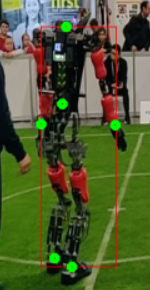
\includegraphics[width=.135\textwidth]{gambar/comp_with_gt/robot_4_gt.png}
  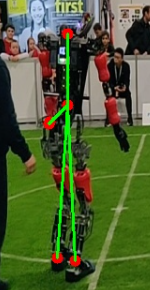
\includegraphics[width=.135\textwidth]{gambar/comp_with_gt/robot_4_res.png} \hfill%
  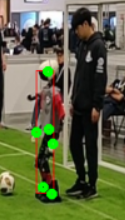
\includegraphics[width=.148\textwidth]{gambar/comp_with_gt/robot_5_gt.png}
  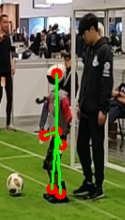
\includegraphics[width=.148\textwidth]{gambar/comp_with_gt/robot_5_res.png} \hfill%
  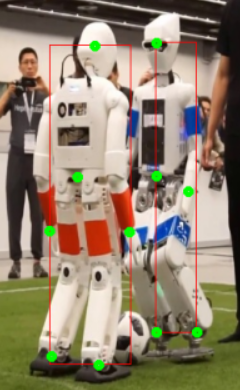
\includegraphics[width=.16\textwidth]{gambar/comp_with_gt/robot_6_gt.png}
  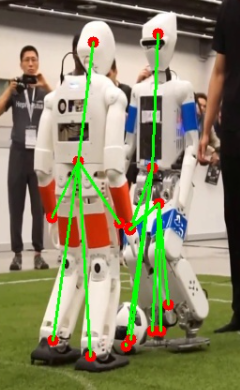
\includegraphics[width=.16\textwidth]{gambar/comp_with_gt/robot_6_res.png}
  \\[\medskipamount]
  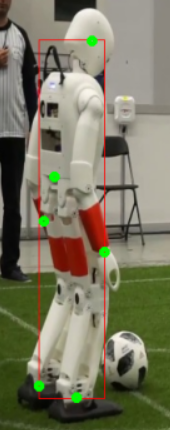
\includegraphics[width=.11\textwidth]{gambar/comp_with_gt/robot_7_gt.png}
  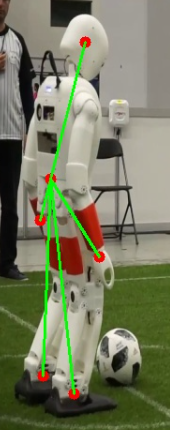
\includegraphics[width=.11\textwidth]{gambar/comp_with_gt/robot_7_res.png} \hfill%
  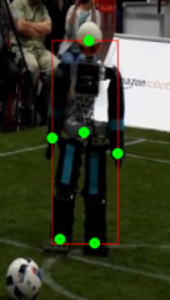
\includegraphics[width=.155\textwidth]{gambar/comp_with_gt/robot_8_gt.png}
  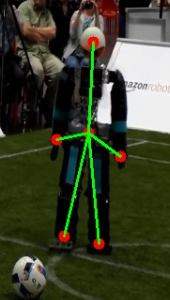
\includegraphics[width=.155\textwidth]{gambar/comp_with_gt/robot_8_res.png} \hfill%
  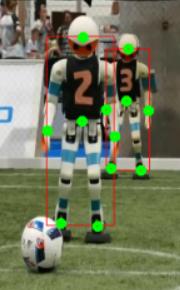
\includegraphics[width=.17\textwidth]{gambar/comp_with_gt/robot_9_gt.png}
  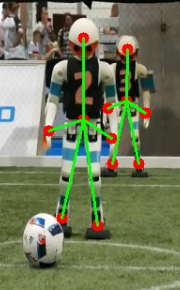
\includegraphics[width=.17\textwidth]{gambar/comp_with_gt/robot_9_res.png}
  \\[\medskipamount]
  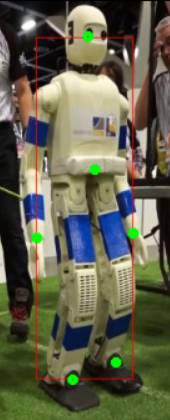
\includegraphics[width=.12\textwidth]{gambar/comp_with_gt/robot_10_gt.png}
  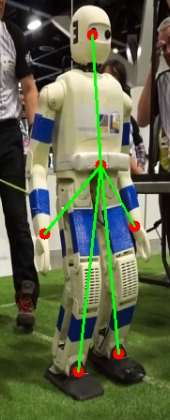
\includegraphics[width=.12\textwidth]{gambar/comp_with_gt/robot_10_res.png} \hfill%
  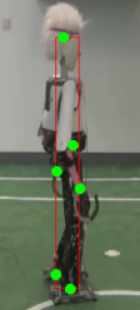
\includegraphics[width=.137\textwidth]{gambar/comp_with_gt/robot_11_gt.png}
  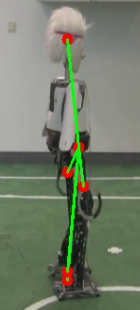
\includegraphics[width=.137\textwidth]{gambar/comp_with_gt/robot_11_res.png} \hfill%
  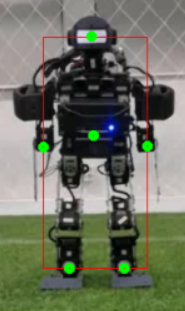
\includegraphics[width=.18\textwidth]{gambar/comp_with_gt/robot_12_gt.png}
  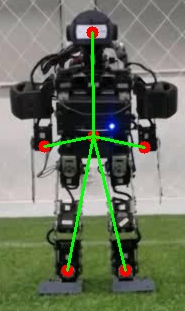
\includegraphics[width=.18\textwidth]{gambar/comp_with_gt/robot_12_res.png}
  \centering
  \captionsetup{justification=centering, margin=2cm}
  \caption{Perbandingan Antara \textit{Ground Truth} dengan Hasil Deteksi pada Setiap Tipe Robot dalam Dataset}
  \label{fig:comparisongtandresult}
\end{figure}